%**************************************************************************************
% License:
% CC BY-NC-SA 4.0 (http://creativecommons.org/licenses/by-nc-sa/4.0/)
%**************************************************************************************

\documentclass[notes]{beamer}

\mode<presentation> {

\usetheme{Madrid}

% Burnt orange
\definecolor{burntorange}{rgb}{0.8, 0.33, 0.0}
\colorlet{beamer@blendedblue}{burntorange}
% Pale yellow
\definecolor{paleyellow}{rgb}{1.0, 1.0, 0.953}
\setbeamercolor{background canvas}{bg=paleyellow}
% Secondary and tertiary palette
\setbeamercolor*{palette secondary}{use=structure,fg=white,bg=burntorange!80!black}
\setbeamercolor*{palette tertiary}{use=structure,fg=white,bg=burntorange!60!black}

% To remove the navigation symbols from the bottom of all slides uncomment this line
%\setbeamertemplate{navigation symbols}{}
}

\usepackage{amsmath}
\DeclareMathOperator*{\argmin}{arg\,min}
\DeclareMathOperator*{\argmax}{arg\,max}
\usepackage{bm}
\usepackage{booktabs} % Allows the use of \toprule, \midrule and \bottomrule in tables
\usepackage{breqn}
\usepackage{cleveref}
\usepackage{graphicx} % for figures
\usepackage[labelsep=space,tableposition=top]{caption}
\renewcommand{\figurename}{Fig.} 
\usepackage{caption,subcaption}% http://ctan.org/pkg/{caption,subcaption}
\usepackage{xcolor}
\usepackage{hyperref}

\AtBeginSection[]{
	\begin{frame}{Outline}
		\tableofcontents[
		currentsection,      % highlight the current section
		hideallsubsections   % show only section titles
		]
	\end{frame}
}

%----------------------------------------------------------------------------------------
%	TITLE PAGE
%----------------------------------------------------------------------------------------
\title[DeepONet: Operator Learning]{DeepONet: Learning Operators with Neural Networks} 
\author{Krishna Kumar} % name
\institute[UT Austin] % institution 
{
University of Texas at Austin \\
\medskip
\textit{
  \url{krishnak@utexas.edu}} % Your email address
}
\date{} % Date, can be changed to a custom date

\begin{document}

\begin{frame}
\titlepage % title page as the first slide
\end{frame}

\begin{frame}
 \frametitle{Overview}
 \tableofcontents
\end{frame}

%----------------------------------------------------------------------------------------
% slides
%----------------------------------------------------------------------------------------

\section{From Functions to Operators: The Conceptual Leap}

%------------------------------------------------
\begin{frame}
\frametitle{Learning Objectives}

\begin{itemize}
    \item Understand the leap from function approximation to operator learning
    \item Master the Universal Approximation Theorem for Operators
    \item Learn the DeepONet architecture: Branch and Trunk networks
    \item Implement operator learning for the derivative operator
    \item Apply DeepONet to the 1D nonlinear Darcy problem
\end{itemize}

\vspace{1cm}
\centering
\href{https://colab.research.google.com/github/kks32-courses/ut-portugal-sciml/blob/main/docs/02-deeponet/deeponet.ipynb}{\beamergotobutton{Open Notebook: DeepONet}}

\end{frame}

%------------------------------------------------
\begin{frame}
\frametitle{The Fundamental Question}

We've learned how neural networks can approximate \textbf{functions}: $f: \mathbb{R}^d \rightarrow \mathbb{R}^m$.

\vspace{1cm}

\begin{alertblock}{But what if we want to learn mappings between infinite-dimensional function spaces?}
Enter \textbf{operators}: mappings that take functions as input and produce functions as output.
\begin{equation*}
\mathcal{G}: \mathcal{A} \rightarrow \mathcal{U}
\end{equation*}
where $\mathcal{A}$ and $\mathcal{U}$ are function spaces.
\end{alertblock}

\textbf{Examples of operators:}
\begin{itemize}
    \item \textbf{Derivative operator:} $\mathcal{G}u = \frac{du}{dx}$
    \item \textbf{Integration operator:} $\mathcal{G}f = \int_0^x f(t) dt$
    \item \textbf{PDE solution operator:} Given boundary conditions or source terms, map to the PDE solution
\end{itemize}

\end{frame}

%------------------------------------------------
\begin{frame}
\frametitle{Traditional Function Approximation}

\textbf{What we're familiar with:}

\begin{columns}[T]
    \begin{column}{0.5\textwidth}
        \textbf{Point-wise mapping:}
        \begin{itemize}
            \item \textbf{Input:} A number $x = 2.5$
            \item \textbf{Output:} A number $f(x) = x^2 = 6.25$
        \end{itemize}
        
        \vspace{0.5cm}
        
        \textbf{Characteristics:}
        \begin{itemize}
            \item Input: Single numbers (scalars)
            \item Output: Single numbers (scalars)
            \item Learn: Point-wise mappings
            \item Architecture: Standard feedforward
        \end{itemize}
    \end{column}
    \begin{column}{0.5\textwidth}
        \begin{figure}[ht]
            \centering
            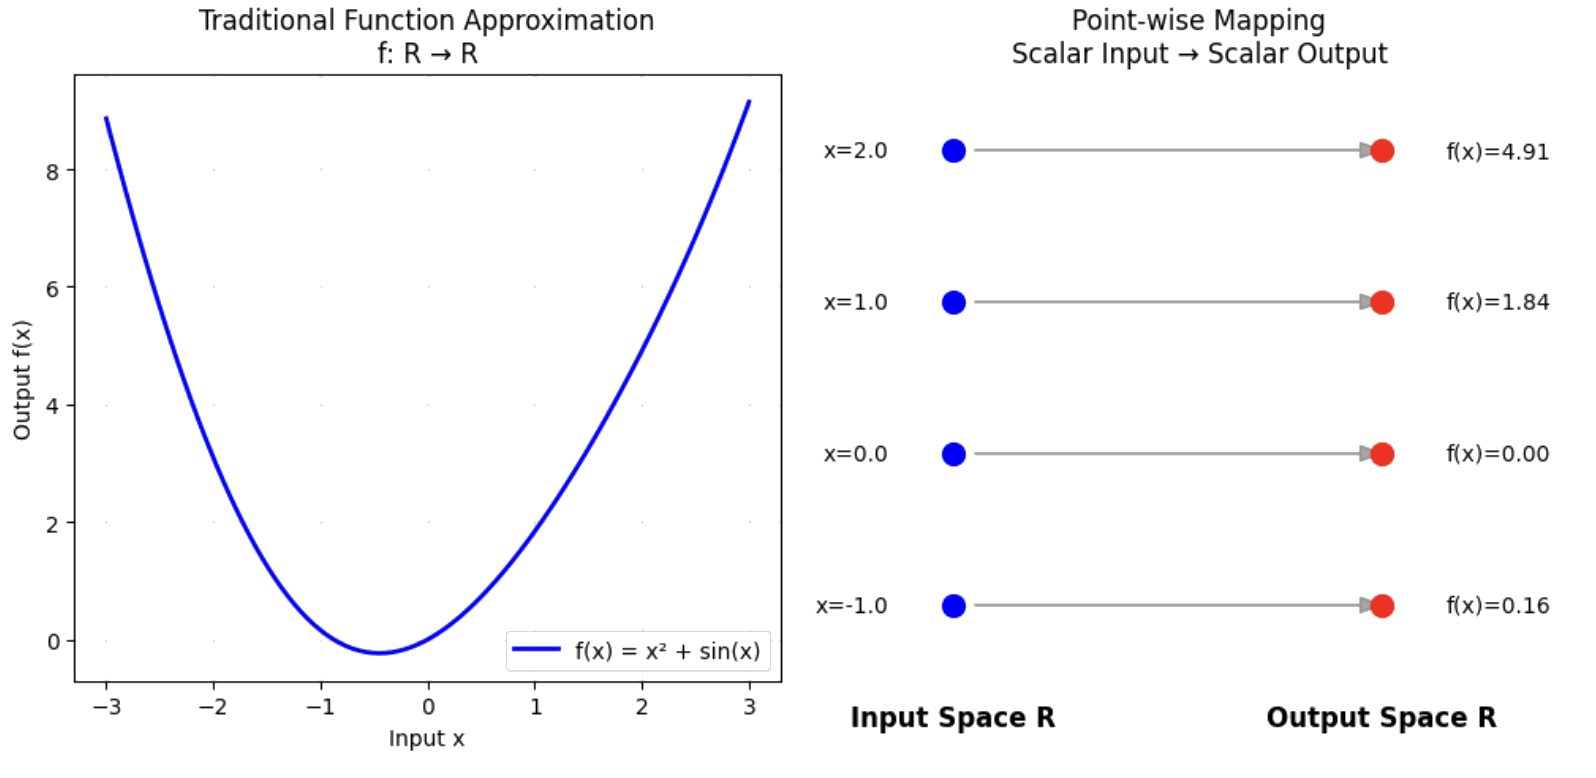
\includegraphics[width=\linewidth]{figs/function_approximation.png}
            \caption*{Traditional neural networks learn scalar-to-scalar mappings.}
        \end{figure}
    \end{column}
\end{columns}

\end{frame}

%------------------------------------------------
\begin{frame}
\frametitle{Operator Learning: The Next Level}

\textbf{The paradigm shift:}

\begin{columns}[T]
    \begin{column}{0.5\textwidth}
        \textbf{Function-to-function mapping:}
        \begin{itemize}
            \item \textbf{Input:} An entire function $u(x) = \sin(x)$
            \item \textbf{Output:} Another entire function $\mathcal{G}[u](x) = \cos(x)$ (the derivative!)
        \end{itemize}
        
        \vspace{0.5cm}
        
        \textbf{Examples in science:}
        \begin{itemize}
            \item $\mathcal{D}[u] = \frac{du}{dx}$ (Differentiation)
            \item $\mathcal{I}[f] = \int_0^x f(t) dt$ (Integration)
            \item $\mathcal{S}[f] = u$ where $\nabla^2 u = f$ (PDE solution)
        \end{itemize}
    \end{column}
    \begin{column}{0.5\textwidth}
        \begin{figure}[ht]
            \centering
            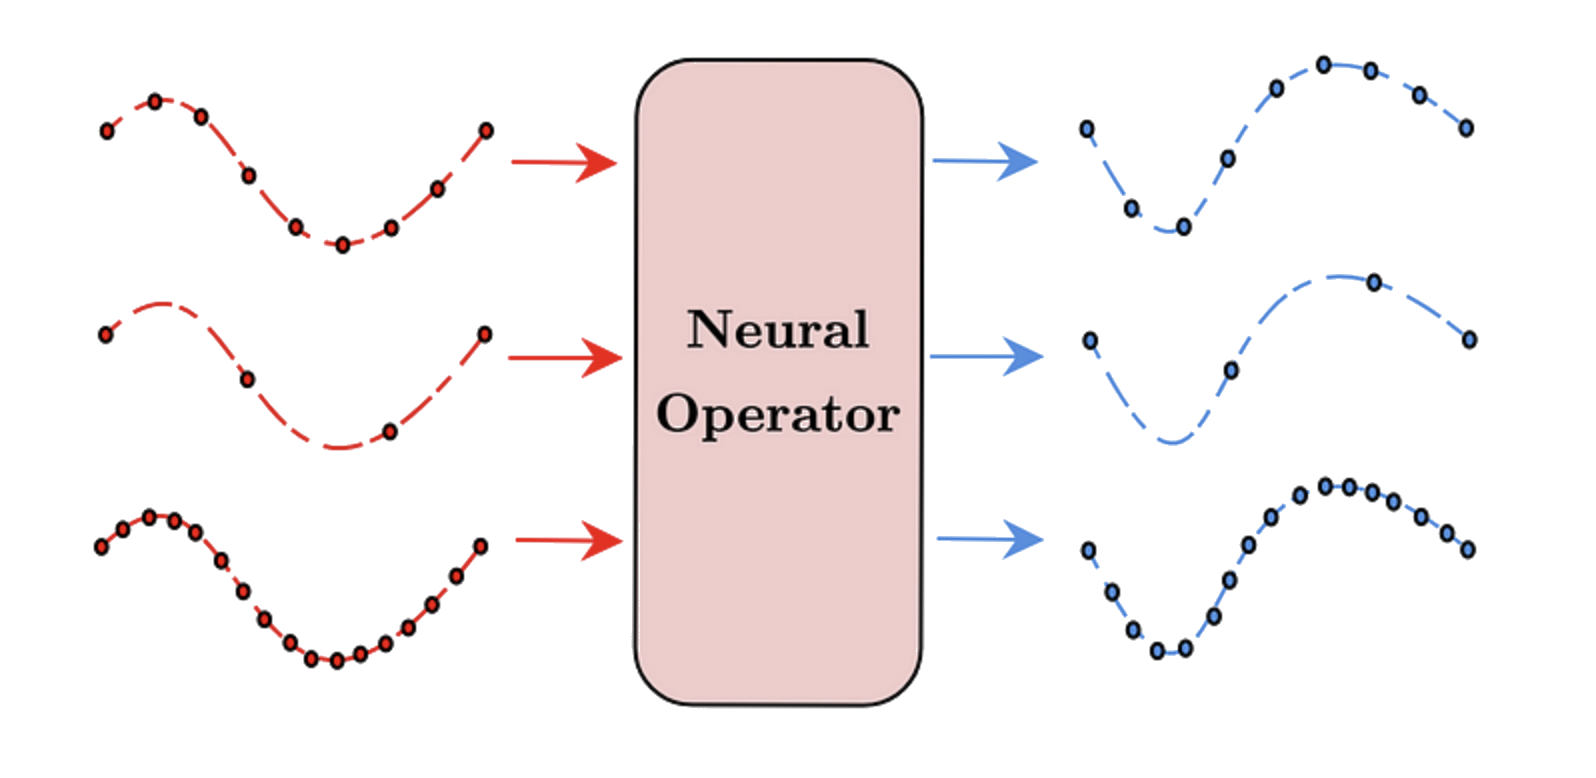
\includegraphics[width=\linewidth]{figs/operator_concept.png}
            \caption*{Operators map entire functions to entire functions.}
        \end{figure}
    \end{column}
\end{columns}

\end{frame}

%------------------------------------------------
\begin{frame}
\frametitle{The Challenge with Traditional Neural Networks}

Standard neural networks learn point-wise mappings: $\mathbb{R}^n \rightarrow \mathbb{R}^m$. But operators map functions to functions.

\begin{alertblock}{Traditional approach limitations:}
\begin{itemize}
    \item \textbf{Fixed discretization:} Networks trained on specific grids can't generalize to different resolutions
    \item \textbf{Curse of dimensionality:} High-dimensional function spaces are computationally intractable
    \item \textbf{No theoretical foundation:} No guarantee that standard networks can approximate operators
\end{itemize}
\end{alertblock}

\textbf{How do we represent infinite-dimensional functions with finite data?}

\vspace{0.5cm}

\textbf{Solution:} We need a fundamentally different architecture that can handle function inputs and outputs while maintaining theoretical guarantees.

\end{frame}

%------------------------------------------------
\section{Universal Approximation Theorem for Operators}

%------------------------------------------------
\begin{frame}
\frametitle{The Breakthrough Theorem}

Just as the Universal Approximation Theorem tells us neural networks can approximate functions, there's a remarkable extension:

\begin{block}{Theorem (Chen \& Chen, 1995)}
Neural networks can approximate \textbf{operators} that map functions to functions!
\end{block}

\textbf{Mathematical Statement:} For any continuous operator $\mathcal{G}: V \subset C(K_1) \rightarrow C(K_2)$ and $\epsilon > 0$, there exist constants such that:

\begin{equation*}
\left|\mathcal{G}(u)(y) - \sum_{k=1}^p \underbrace{\sum_{i=1}^n c_i^k \sigma\left(\sum_{j=1}^m \xi_{ij}^k u(x_j) + \theta_i^k\right)}_{\text{Branch Network}} \underbrace{\sigma(w_k \cdot y + \zeta_k)}_{\text{Trunk Network}}\right| < \epsilon
\end{equation*}

\end{frame}

%------------------------------------------------
\begin{frame}
\frametitle{Decoding the Theorem}

This looks complex, but the insight is beautiful:

\begin{enumerate}
    \item \textbf{Branch Network:} Processes function $u$ sampled at sensor points $\{x_j\}$
    \item \textbf{Trunk Network:} Processes output coordinates $y$
    \item \textbf{Combination:} Multiply branch and trunk outputs, then sum
\end{enumerate}

\begin{block}{Key insight}
Any operator can be written as:
\begin{equation*}
\mathcal{G}(u)(y) \approx \sum_{k=1}^p b_k(u) \cdot t_k(y)
\end{equation*}
where $b_k$ depends only on the input function and $t_k$ depends only on the output location!
\end{block}

This decomposition is the theoretical foundation for the DeepONet architecture.

\end{frame}

%------------------------------------------------
\section{DeepONet Architecture}

%------------------------------------------------
\begin{frame}
\frametitle{DeepONet: The Practical Implementation}

\textbf{DeepONet} (Deep Operator Network) is the practical implementation of the Operator Universal Approximation Theorem.

\begin{block}{Core Architecture}
\begin{equation*}
\mathcal{G}_\theta(u)(y) = \sum_{k=1}^p b_k(u) \cdot t_k(y) + b_0
\end{equation*}
where:
\begin{itemize}
    \item \textbf{Branch network:} $b_k(u) = \mathcal{B}_k([u(x_1), u(x_2), \ldots, u(x_m)])$
    \item \textbf{Trunk network:} $t_k(y) = \mathcal{T}_k(y)$
    \item \textbf{$p$:} Number of basis functions (typically 50-200)
    \item \textbf{$b_0$:} Bias term
\end{itemize}
\end{block}

\end{frame}

%------------------------------------------------
\begin{frame}
\frametitle{DeepONet Architecture Diagram}

\begin{figure}[ht]
	\centering
	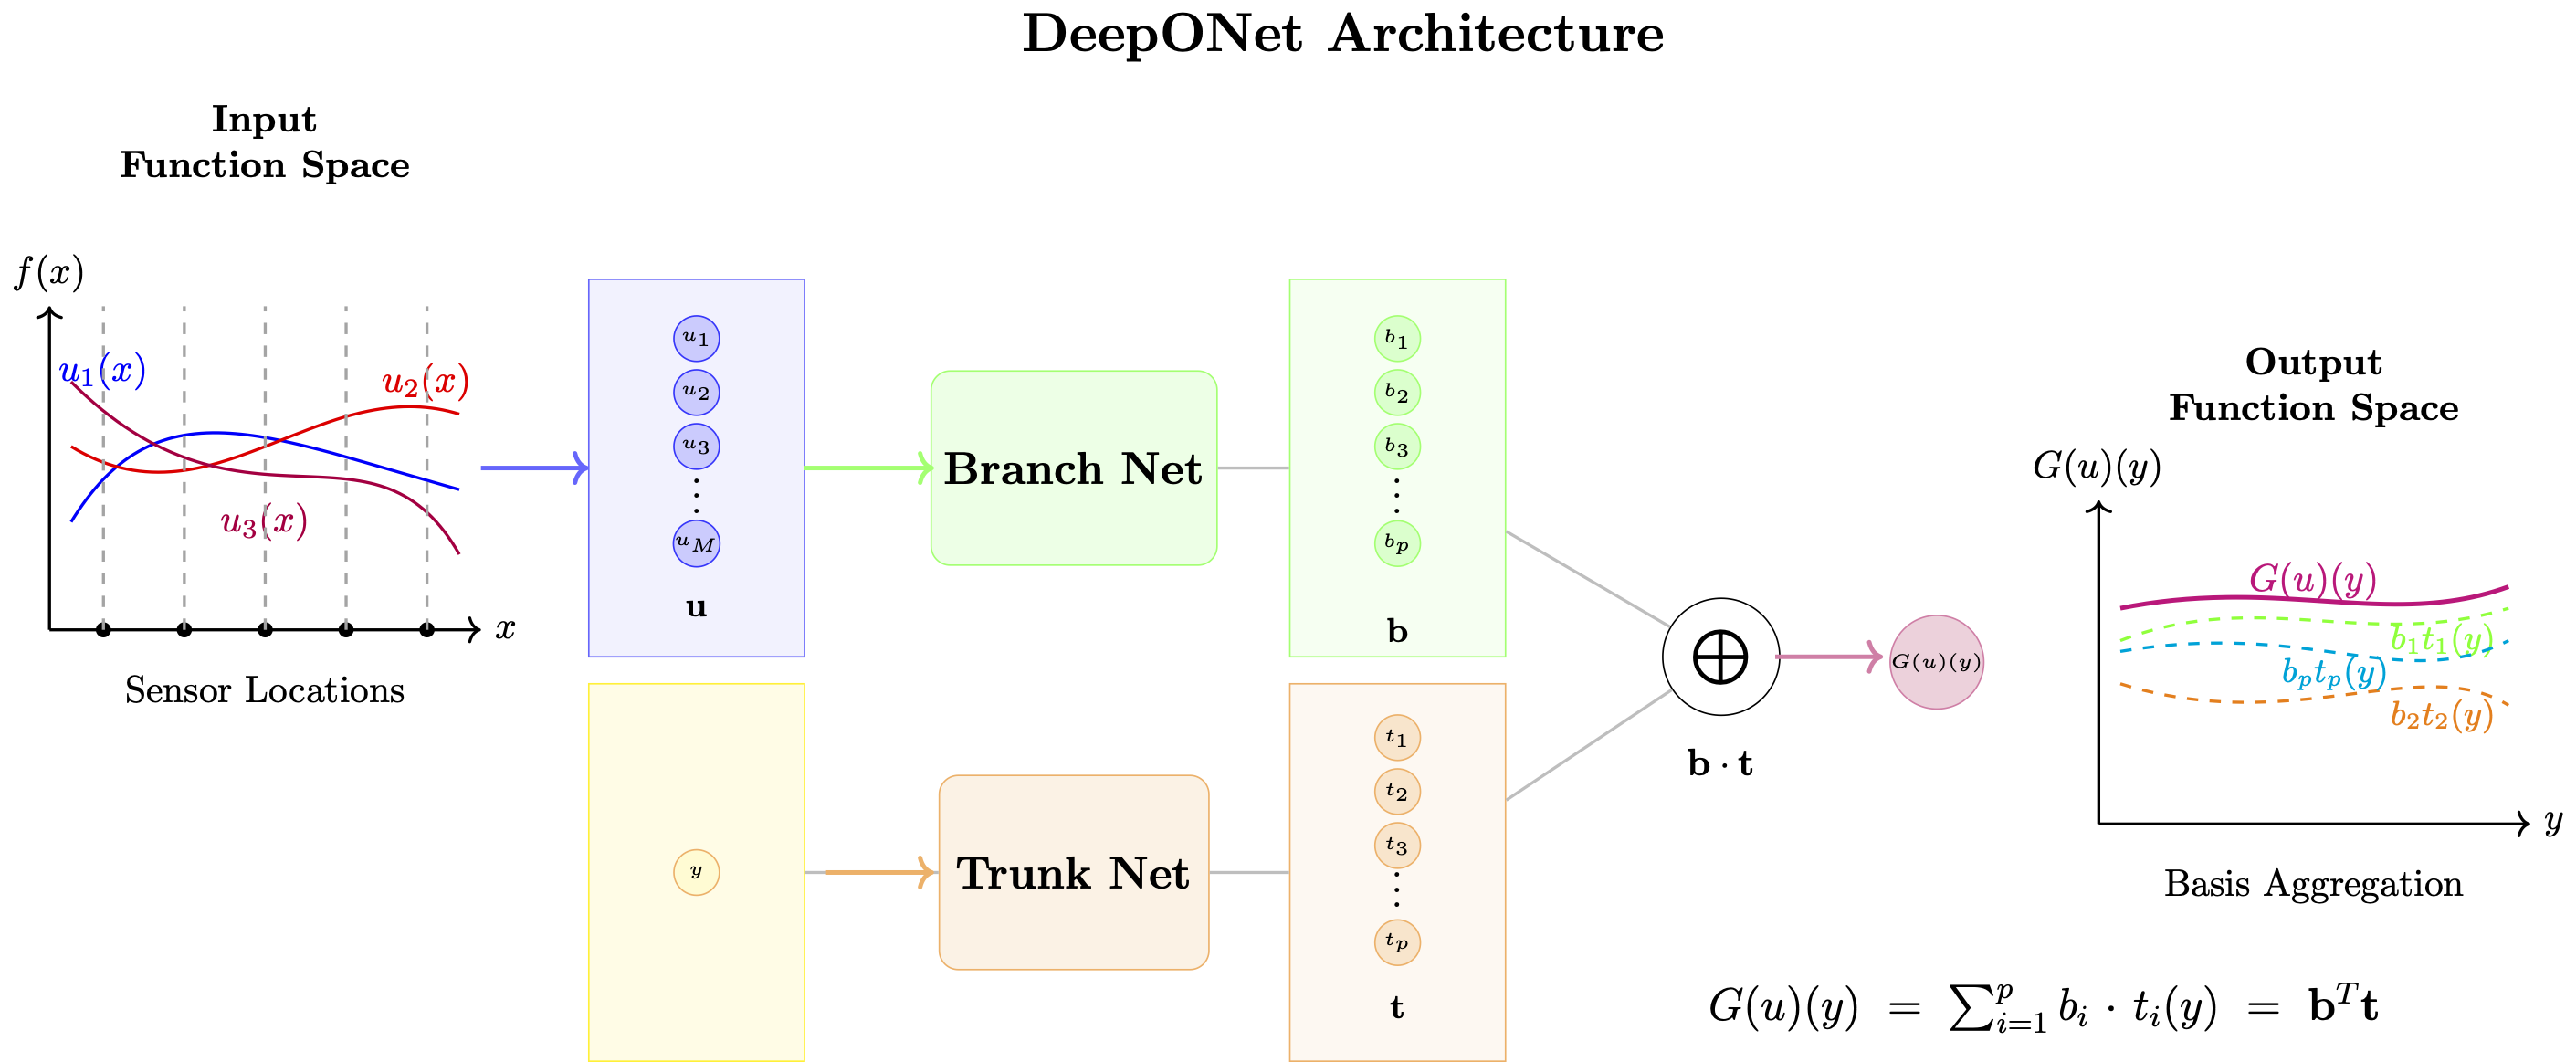
\includegraphics[width=0.8\textwidth]{figs/deeponet-arch.png}
	\caption*{DeepONet architecture showing branch and trunk networks.}
\end{figure}

\textbf{Data flow:}
\begin{enumerate}
    \item Input function $u$ sampled at sensor points → Branch network → Coefficients $\{b_k\}$
    \item Query points $y$ → Trunk network → Basis functions $\{t_k\}$  
    \item Element-wise multiplication and summation → Output $\mathcal{G}(u)(y)$
\end{enumerate}

\end{frame}

%------------------------------------------------
\begin{frame}
\frametitle{Training Data Structure and Loss Function}

\textbf{Input-output pairs:} $(u^{(i)}, y^{(j)}, \mathcal{G}(u^{(i)})(y^{(j)}))$

\begin{itemize}
    \item \textbf{$N$} input functions: $\{u^{(i)}\}_{i=1}^N$
    \item Each function sampled at \textbf{$m$} sensors: $\{u^{(i)}(x_j)\}_{j=1}^m$
    \item Corresponding outputs at \textbf{query points}: $\{\mathcal{G}(u^{(i)})(y_k)\}$
\end{itemize}

\begin{block}{Loss Function}
\begin{equation*}
\mathcal{L}(\theta) = \frac{1}{N \cdot P} \sum_{i=1}^N \sum_{k=1}^P \left|\mathcal{G}_\theta(u^{(i)})(y_k) - \mathcal{G}(u^{(i)})(y_k)\right|^2
\end{equation*}
\end{block}

\textbf{Key Advantages:}
\begin{itemize}
    \item \textbf{Resolution independence:} Train on one grid, evaluate on any grid
    \item \textbf{Fast evaluation:} Once trained, instant prediction (no iterative solving)
    \item \textbf{Generalization:} Works for new functions not seen during training
\end{itemize}

\end{frame}

%------------------------------------------------
\section{Example 1: The Derivative Operator}

%------------------------------------------------
\begin{frame}
\frametitle{Perfect Starting Point: Learning Derivatives}

\textbf{Problem Setup:} Learn the derivative operator $\mathcal{D}[u] = \frac{du}{dx}$

\begin{columns}[T]
    \begin{column}{0.5\textwidth}
        \textbf{Why this example:}
        \begin{itemize}
            \item Simple and intuitive
            \item Exact analytical solution for verification
            \item Shows how DeepONet learns basis decompositions
            \item Bridges function approximation → operator learning
        \end{itemize}
        
        \vspace{0.5cm}
        
        \textbf{Input functions:} Cubic polynomials
        \begin{equation*}
        u(x) = ax^3 + bx^2 + cx + d
        \end{equation*}
        
        \textbf{Target operator:}
        \begin{equation*}
        \mathcal{D}[u](x) = 3ax^2 + 2bx + c
        \end{equation*}
    \end{column}
    \begin{column}{0.5\textwidth}
        \begin{figure}[ht]
            \centering
            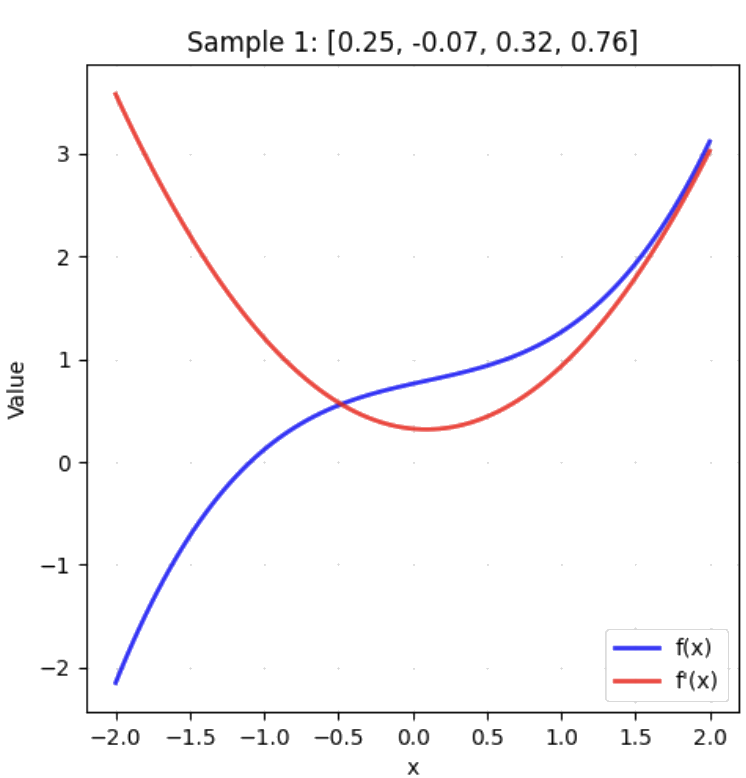
\includegraphics[width=\linewidth]{figs/polynomial_samples.png}
            \caption*{Sample cubic polynomials and their derivatives.}
        \end{figure}
    \end{column}
\end{columns}

\end{frame}

%------------------------------------------------
\begin{frame}
\frametitle{The DeepONet Challenge}

\textbf{Key insight:} The derivative of a cubic is always quadratic, so it can be written as:
\begin{equation*}
\frac{du}{dx} = w_1 \cdot 1 + w_2 \cdot x + w_3 \cdot x^2
\end{equation*}
where $w_1 = c$, $w_2 = 2b$, $w_3 = 3a$.

\vspace{1cm}

\begin{alertblock}{The DeepONet challenge}
Can it learn this mapping automatically without being told the explicit form?
\end{alertblock}

\vspace{0.5cm}

\textbf{What we expect:} 
\begin{itemize}
    \item Branch network should learn to extract coefficients $\{a, b, c\}$
    \item Trunk network should learn basis functions $\{1, x, x^2\}$
    \item The combination should reproduce the derivative exactly
\end{itemize}

\end{frame}


%------------------------------------------------
\begin{frame}
\frametitle{Prediction Results}

\begin{figure}[ht]
	\centering
	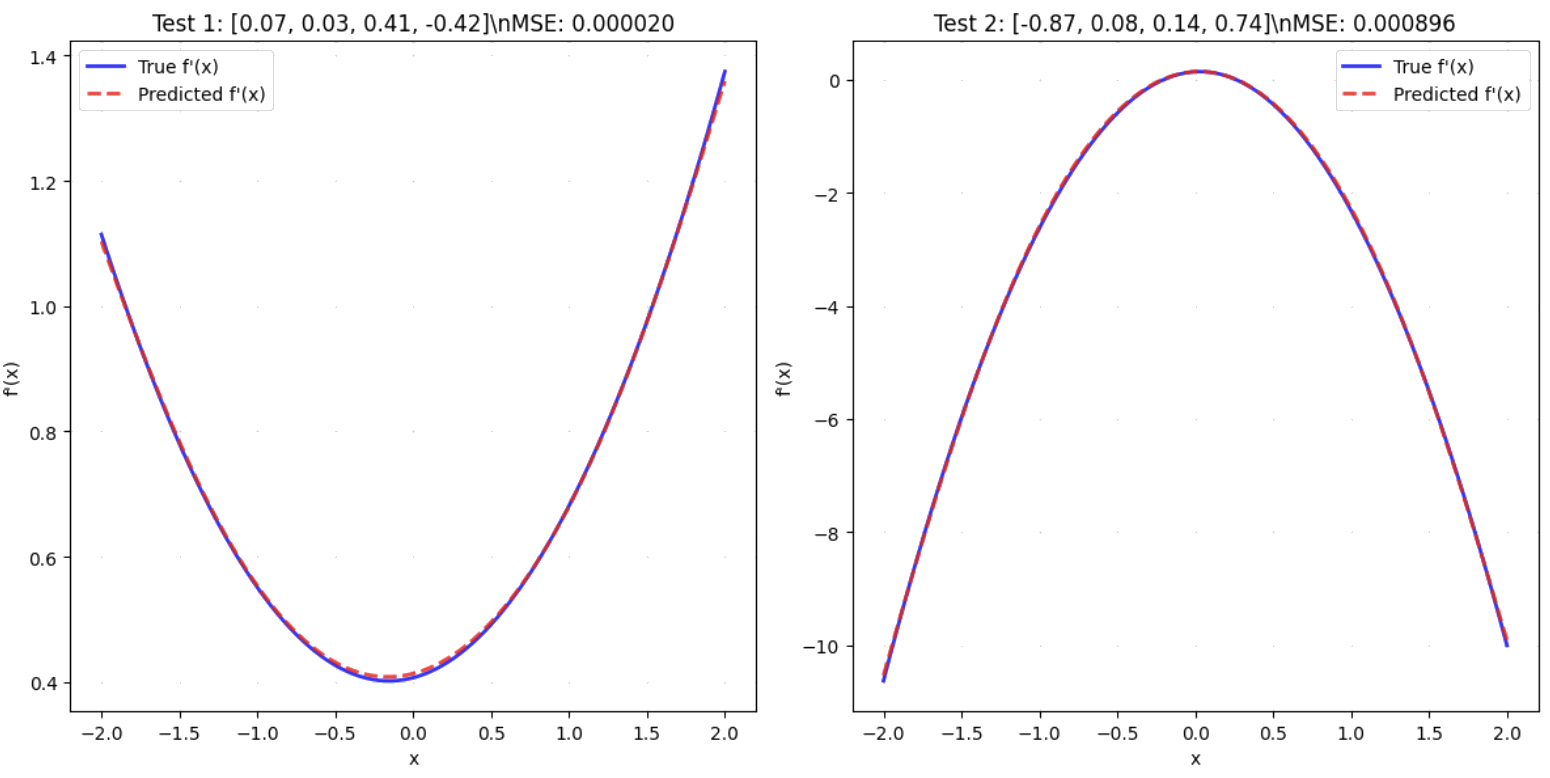
\includegraphics[width=\textwidth]{figs/prediction_results.png}
	\caption*{DeepONet predictions vs. true derivatives for test polynomials.}
\end{figure}

\textbf{Results:}
\begin{itemize}
    \item Perfect agreement between predicted and true derivatives
    \item Works for polynomial coefficients not seen during training
    \item Demonstrates true operator learning, not just pattern memorization
\end{itemize}

\end{frame}

%------------------------------------------------
\begin{frame}
\frametitle{Understanding What DeepONet Learned}

\begin{figure}[ht]
	\centering
	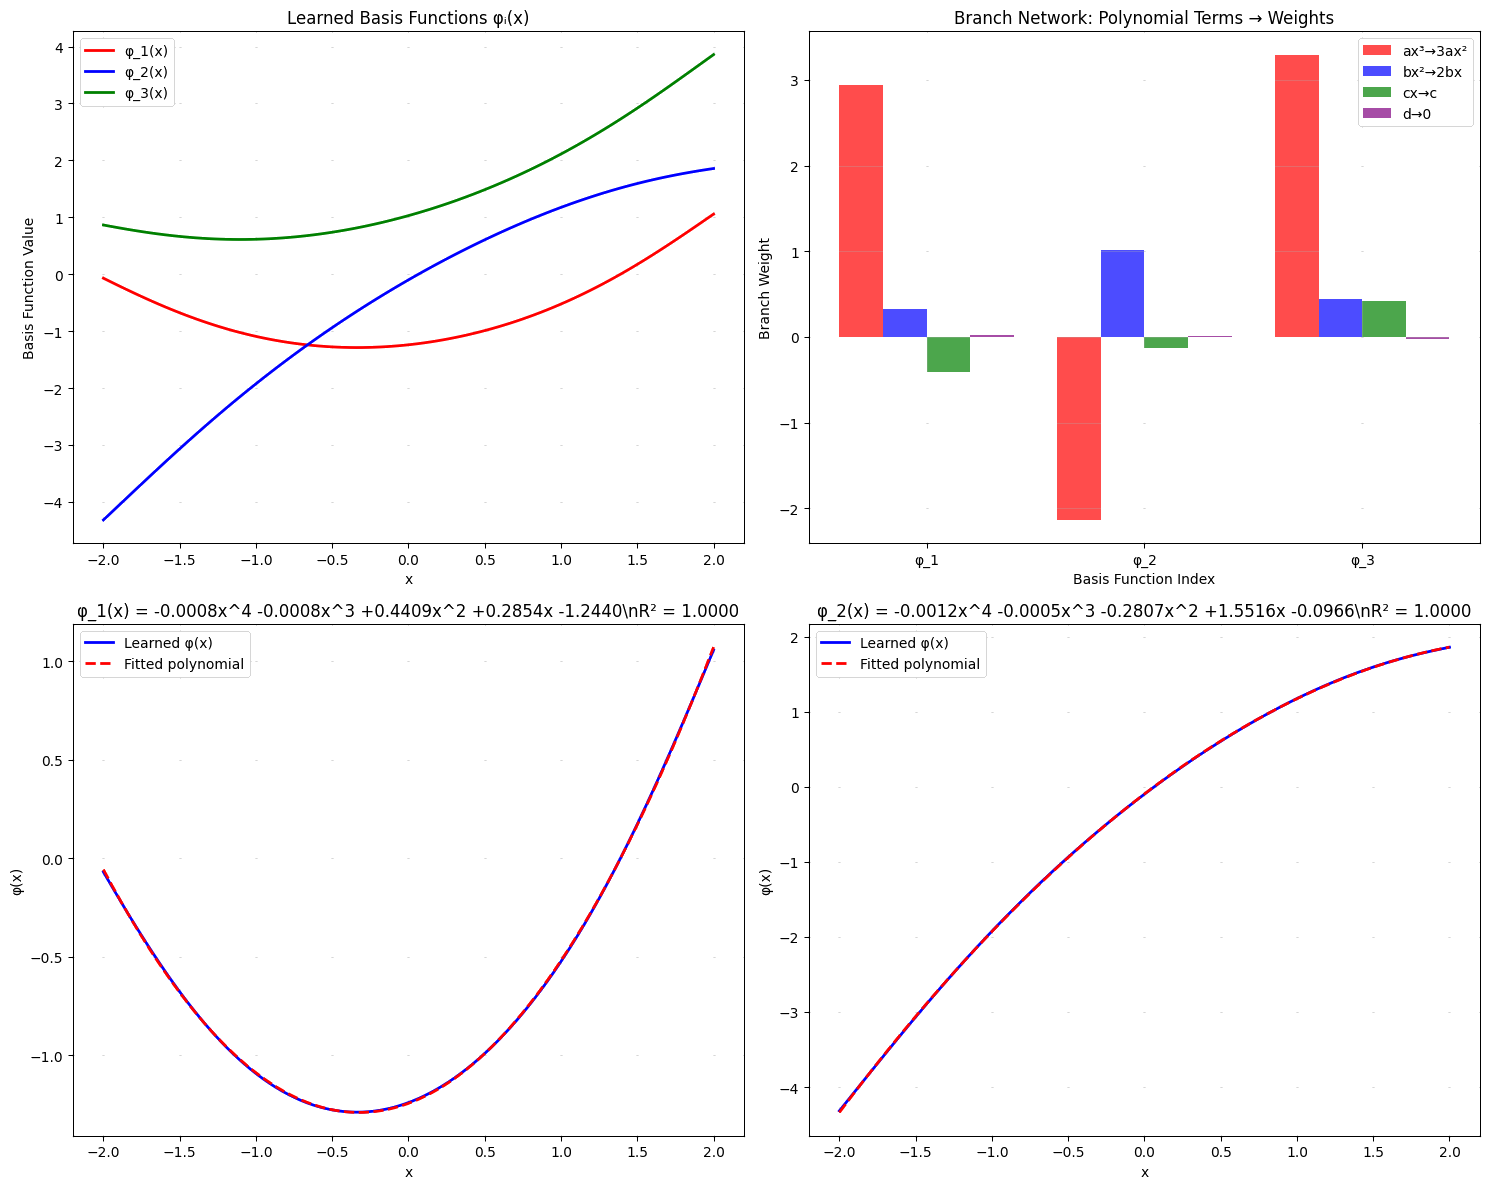
\includegraphics[width=\textwidth]{figs/basis_analysis.png}
	\caption*{Analysis of learned basis functions and branch network behavior.}
\end{figure}

\textbf{Mathematical Decomposition:}
\begin{equation*}
f'(x) \approx \sum_{i=1}^3 w_i(a,b,c,d) \times \phi_i(x) + \text{bias}
\end{equation*}

\textbf{Key findings:}
\begin{itemize}
    \item Basis functions $\phi_i(x)$ approximate $\{1, x, x^2\}$
    \item Branch network learns to map coefficients to appropriate weights
    \item The decomposition matches the analytical structure perfectly
\end{itemize}

\end{frame}

%------------------------------------------------
\section{Example 2: The 1D Nonlinear Darcy Problem}

%------------------------------------------------
\begin{frame}
\frametitle{A Real PDE: The 1D Nonlinear Darcy Problem}

\textbf{Now for something more challenging:} A real PDE with nonlinear physics!

\begin{block}{Problem Formulation}
The 1D nonlinear Darcy equation models groundwater flow with solution-dependent permeability:
\begin{equation*}
\frac{d}{dx}\left(-\kappa(u(x))\frac{du}{dx}\right) = f(x), \quad x \in [0,1]
\end{equation*}
where:
\begin{itemize}
    \item $u(x)$ is the \textbf{solution field} (pressure/hydraulic head)
    \item $\kappa(u) = 0.2 + u^2(x)$ is the \textbf{nonlinear permeability}
    \item $f(x) \sim \text{GP}(0, k(x, x'))$ is a \textbf{Gaussian random field source}
    \item Homogeneous Dirichlet BCs: $u(0) = 0$, $u(1) = 0$
\end{itemize}
\end{block}

\end{frame}

%------------------------------------------------
\begin{frame}
\frametitle{The Operator Learning Challenge}

\textbf{Goal:} Learn the solution operator $\mathcal{G}$ such that:
\begin{equation*}
\mathcal{G}[f] = u
\end{equation*}
where $u$ is the solution to the nonlinear Darcy equation for source $f$.

\vspace{1cm}

\begin{alertblock}{Why this is much harder than the derivative operator:}
\begin{enumerate}
    \item \textbf{Nonlinear PDE:} No analytical solution
    \item \textbf{Random sources:} Infinite variety of input functions  
    \item \textbf{Complex physics:} Solution depends on entire source profile
\end{enumerate}
\end{alertblock}

\vspace{0.5cm}

\textbf{Traditional approach:} For each new source $f$, solve the PDE numerically (expensive!)

\textbf{DeepONet approach:} Learn the operator once, then instant evaluation for any new source

\end{frame}

%------------------------------------------------
\begin{frame}
\frametitle{Darcy Dataset Generation}

\begin{figure}[ht]
	\centering
	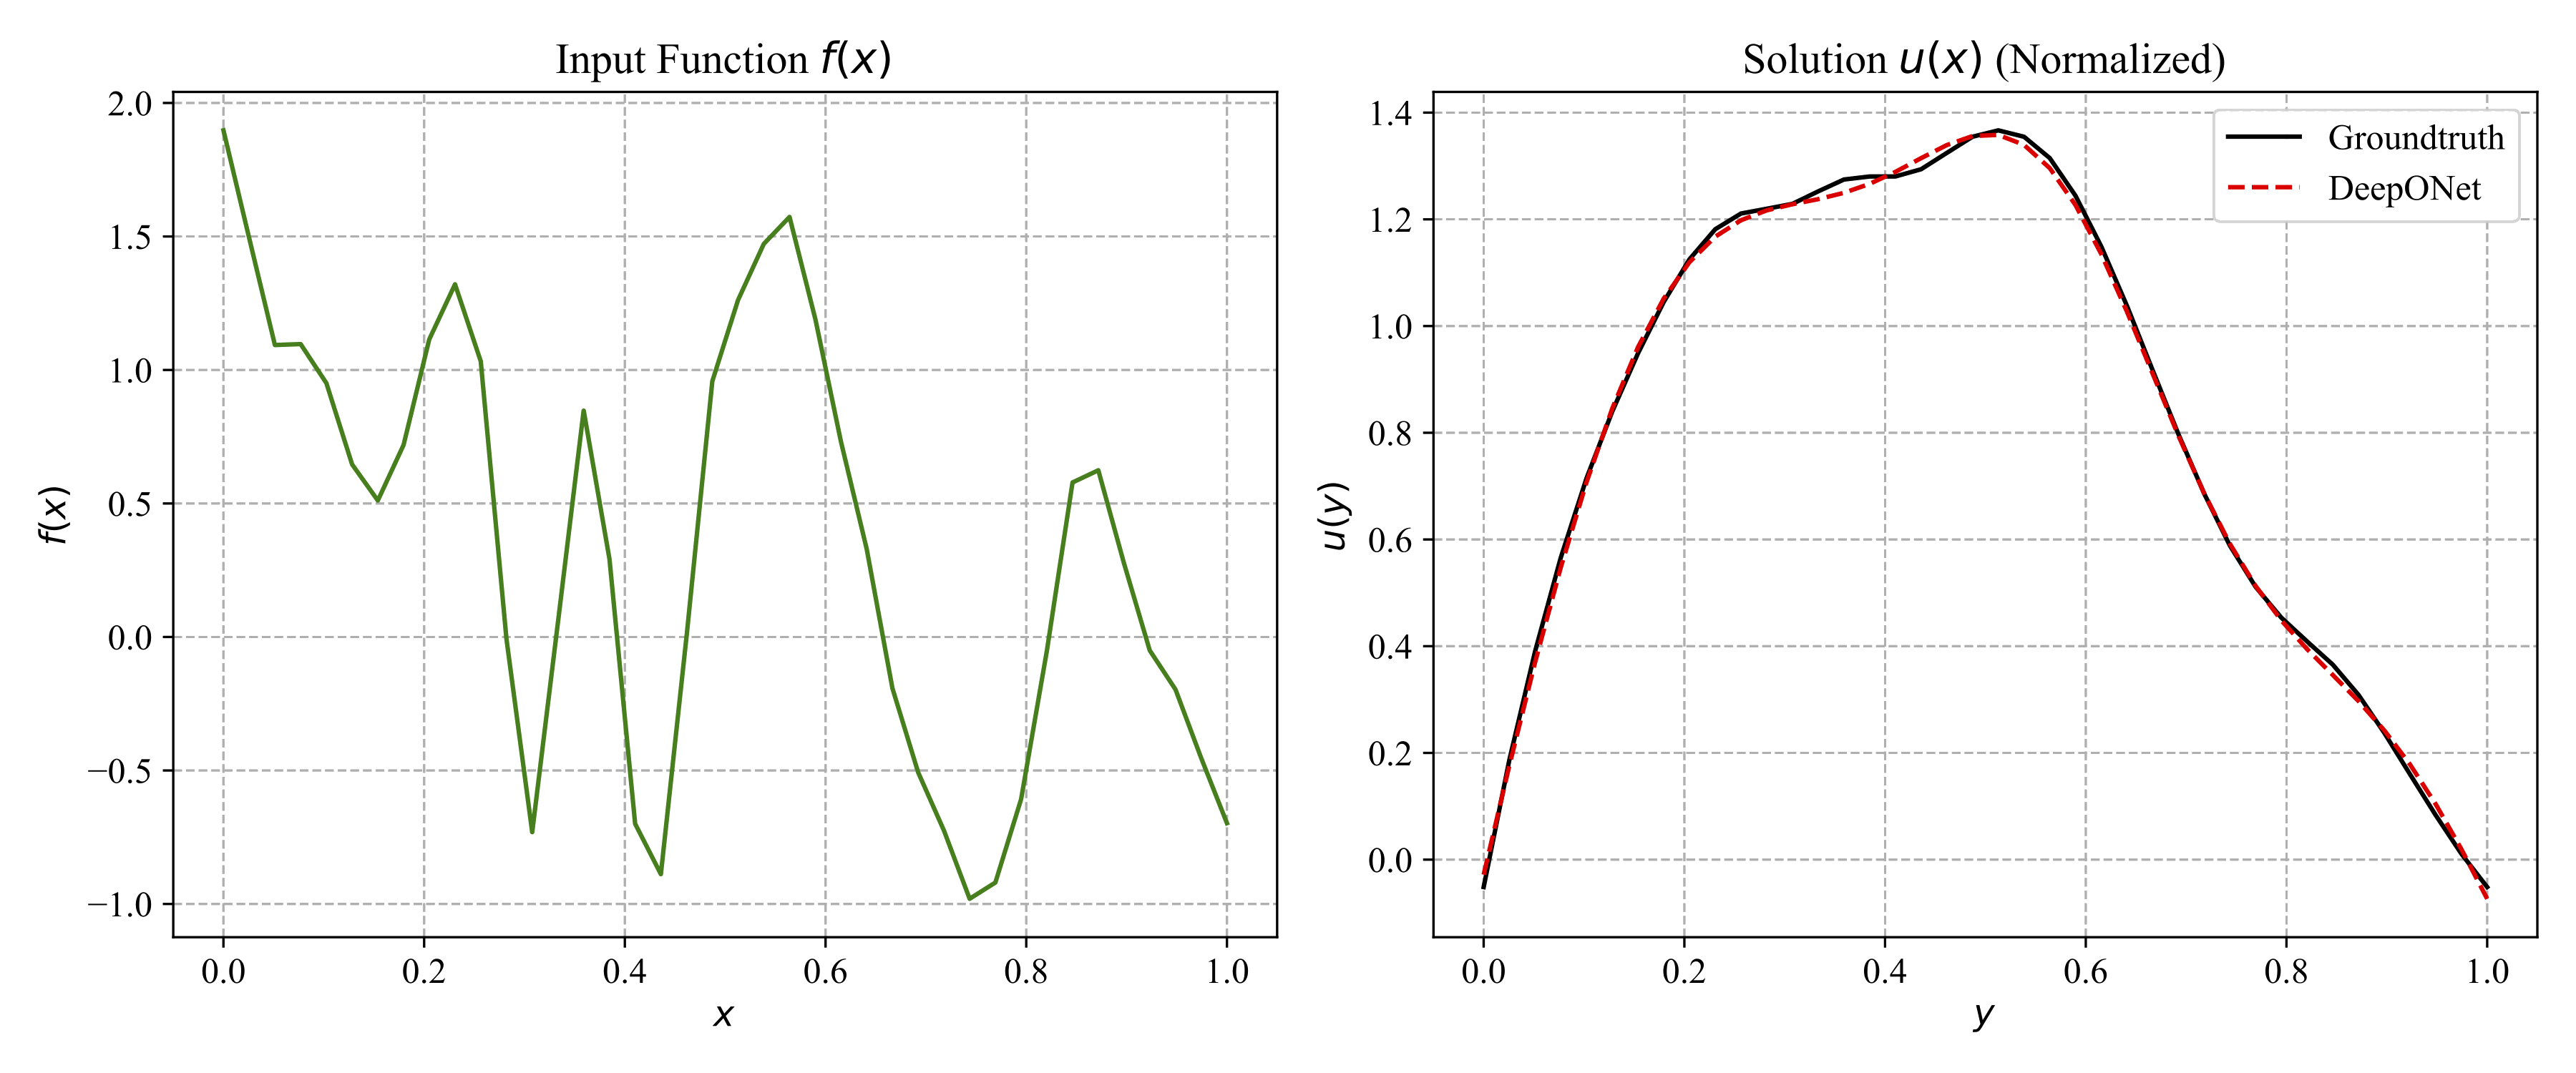
\includegraphics[width=\textwidth]{figs/darcy_samples.png}
	\caption*{Sample Gaussian random field sources and their corresponding solutions.}
\end{figure}

\textbf{Dataset characteristics:}
\begin{itemize}
    \item 1000 source functions $f(x)$ generated from a Gaussian process
    \item Each source solved numerically using iterative methods
    \item Solutions exhibit complex, nonlinear relationships to sources
    \item Provides rich training data for operator learning
\end{itemize}

\end{frame}

%------------------------------------------------
\begin{frame}
\frametitle{Learned Basis Functions for Darcy}

\begin{figure}[ht]
	\centering
	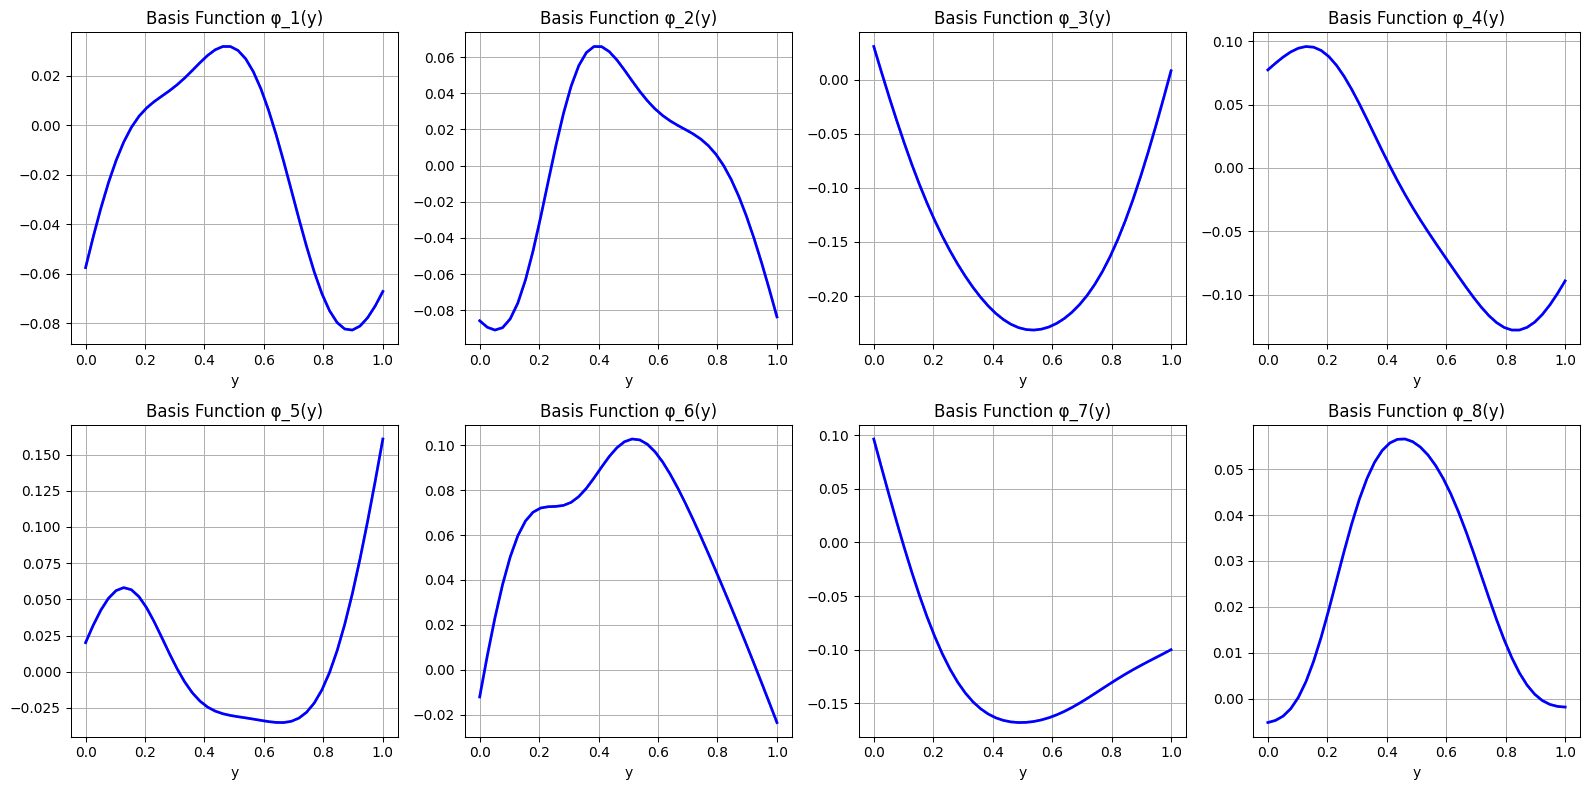
\includegraphics[width=\textwidth]{figs/darcy_basis_functions.png}
	\caption*{First 8 basis functions learned by the trunk network.}
\end{figure}

\textbf{Observations:}
\begin{itemize}
    \item Basis functions capture diverse spatial patterns
    \item Some functions emphasize boundary behavior
    \item Others capture interior oscillations
    \item Together they span the solution space for the nonlinear Darcy operator
\end{itemize}

\end{frame}

%------------------------------------------------
\section{Summary and Implications}

%------------------------------------------------
\begin{frame}
\frametitle{What We've Learned: The Paradigm Shift}

\begin{block}{1. Conceptual Leap}
\begin{itemize}
    \item \textbf{Functions:} $\mathbb{R}^d \rightarrow \mathbb{R}^m$ (point to point)
    \item \textbf{Operators:} $\mathcal{F}_1 \rightarrow \mathcal{F}_2$ (function to function)
\end{itemize}
\end{block}

\begin{block}{2. Theoretical Foundation}
\begin{itemize}
    \item Universal Approximation Theorem for Operators
    \item Branch-trunk architecture emerges naturally
    \item Basis function decomposition: $\mathcal{G}(u)(y) = \sum_k b_k(u) \cdot t_k(y)$
\end{itemize}
\end{block}

\begin{block}{3. Practical Implementation}
\begin{itemize}
    \item \textbf{Branch network:} Encodes input functions into coefficients
    \item \textbf{Trunk network:} Generates basis functions at query points
    \item \textbf{Training:} Learn from input-output function pairs
\end{itemize}
\end{block}

\end{frame}

%------------------------------------------------
\begin{frame}
\frametitle{Key Advantages of DeepONet}

\begin{itemize}
	\item \textbf{Resolution independence:} Train on one grid, evaluate on any grid
    \item \textbf{Fast evaluation:} Once trained, instant prediction
    \item \textbf{Generalization:} Works for new functions not seen during training  
    \item \textbf{Physical consistency:} Learns the underlying operator, not just patterns
\end{itemize}

\vspace{1cm}

\begin{block}{DeepONet represents a paradigm shift:}
\begin{itemize}
    \item \textbf{Traditional numerical methods:} Solve each problem instance
    \item \textbf{Operator learning:} Learn the solution pattern once, apply everywhere
\end{itemize}
\end{block}
\end{frame}

%------------------------------------------------
\begin{frame}
\frametitle{When to Use DeepONet}

\begin{block}{Ideal scenarios:}
\begin{itemize}
    \item \textbf{Parametric PDEs:} Need solutions for many different source terms/boundary conditions
    \item \textbf{Real-time applications:} Require instant evaluation
    \item \textbf{Complex geometries:} Traditional methods struggle
    \item \textbf{Multi-query problems:} Same operator, many evaluations
\end{itemize}
\end{block}

\begin{alertblock}{Limitations:}
\begin{itemize}
    \item \textbf{Training data:} Need many solved examples
    \item \textbf{Complex operators:} Very nonlinear mappings may be challenging
    \item \textbf{High dimensions:} Curse of dimensionality still applies
\end{itemize}
\end{alertblock}

\end{frame}

%------------------------------------------------
\begin{frame}
\frametitle{The Bigger Picture}

This opens new possibilities for:

\begin{columns}[T]
    \begin{column}{0.5\textwidth}
        \textbf{Scientific Applications:}
        \begin{itemize}
            \item \textbf{Inverse problems:} Learn parameter-to-solution mappings
            \item \textbf{Control applications:} Real-time system response
            \item \textbf{Multi-physics:} Coupled operator learning
            \item \textbf{Scientific discovery:} Understanding operator structure
        \end{itemize}
    \end{column}
    \begin{column}{0.5\textwidth}
        \textbf{Future Directions:}
        \begin{itemize}
            \item \textbf{Multi-output operators:} Vector-valued mappings
            \item \textbf{Higher dimensions:} 2D/3D PDEs
            \item \textbf{Physics-informed training:} Incorporate governing equations
            \item \textbf{Fourier Neural Operators:} Alternative architectures
        \end{itemize}
    \end{column}
\end{columns}

\vspace{1cm}

\begin{center}
\textbf{Next:} Combine with PINNs for physics-informed operator learning!
\end{center}

\end{frame}

%------------------------------------------------
\begin{frame}
\frametitle{Questions?}

\centering
\Large Thank you!

\vspace{2cm}

\textbf{Contact:} \\
Krishna Kumar \\
\textit{krishnak@utexas.edu} \\
University of Texas at Austin

\vspace{1cm}

\textbf{Interactive Demo:} \\
\href{https://colab.research.google.com/github/kks32-courses/ut-portugal-sciml/blob/main/docs/02-deeponet/deeponet.ipynb}{\beamergotobutton{DeepONet Notebook}}

\end{frame}

\end{document}